\documentclass[11pt,UTF8]{ctexart}
\usepackage{setspace}
\usepackage{geometry}
\usepackage{amsthm,amsmath,amsfonts,amssymb}%\because\therefore
\usepackage{mathtools}%underset
\usepackage{cancel}
\usepackage{extarrows}
\usepackage{enumerate}
\usepackage{tikz,tikz-cd,forest}
\usepackage{float}
\usepackage{gensymb}
\usepackage{url}
\usepackage[unicode=true,%本行非常重要 支持中文目录hyperref CJKbookmarks对二级目录没用
	colorlinks,
	linkcolor=black,
	anchorcolor=black,
	citecolor=black,
	CJKbookmarks=false]{hyperref}
\usepackage{datetime}
\newdateformat{builddatemonth}{\THEYEAR.\twodigit{\THEMONTH}}
\newdateformat{builddate}{\THEYEAR\twodigit{\THEMONTH}\twodigit{\THEDAY}}

\newtheorem{theorem}{定理}
\newtheorem{definition}{定义}
\newtheorem{example}{例}%*去除编号
\newtheorem*{analysis}{分析}
\newtheorem{corollary}{推论}
\newtheorem*{corollary_convex}{推论}
\newtheorem{exercise}{练习}
\geometry{top=20mm,bottom=20mm,left=20mm,right=20mm}
\pagestyle{plain}%删除页眉

\def\zz{\mathbb{Z}}
\def\rr{\mathbb{R}}
\def\diff{\,\mathrm{d}}
\def\mmid{\enspace\Big|\enspace}
\def\eps{\varepsilon}
\def\disp{\displaystyle}
\newcommand{\ssum}[1]{\displaystyle\sum_{n=1}^{\infty}#1}
\newcommand{\ssumz}[1]{\displaystyle\sum_{n=0}^{\infty}#1}
\newcommand{\ssumk}[1]{\displaystyle\sum_{k=1}^{\infty}#1}
\newcommand{\ssumkn}[1]{\displaystyle\sum_{k=1}^{n}#1}
\newcommand{\limtoinf}[1]{\displaystyle\lim_{n\to\infty}#1}
\newcommand{\intab}[3]{\displaystyle\int_{#1}^{#2}{#3}\,\diff x}
\newcommand{\intabu}[4]{\displaystyle\int_{#1}^{#2}{#3}\,\diff #4}
\newcommand{\inpro}[1]{\langle #1\rangle}
\newcommand{\lrp}[1]{\left(#1\right)}
\newcommand{\lra}[1]{\left|#1\right|}
\newcommand{\nums}[1]{\{#1\}}
\newcommand{\floor}[1]{\lfloor#1\rfloor}
\newcommand{\ol}[1]{\mathop{\overline{#1}}}%\mathop important!!!

\usetikzlibrary{graphs}
\usetikzlibrary{automata}

\renewcommand{\thefootnote}{\fnsymbol{footnote}}

\title{数字电路与逻辑设计笔记}
\author{陈鸿峥}
\date{{\builddatemonth\today} \footnote{\text{Build \builddate\today}}}%加了build

\begin{document}

\maketitle
\renewcommand{\thefootnote}{\arabic{footnote}}
\setcounter{footnote}{0}

\setcounter{tocdepth}{2}%设置深度
\tableofcontents

\section{概述}
\begin{enumerate}
	\item 目的:系统掌握数字系统的基本概念、思维模式与设计方法,帮助深入理解计算机架构
	\item 应用:
	\begin{itemize}
		\item 人工智能+GPU/FPGA
		\item 云计算+FPGA
		\item 物联网+传感硬件系统
		\item 软件定义网络系统
	\end{itemize}
\end{enumerate}


\section{基本概念}
\subsection{数字与模拟}
\begin{enumerate}
	\item 数字(digital)量:离散值,01
	\item 模拟(analog)量:连续值
\end{enumerate}

\subsection{数的表示}
\subsubsection{进制(system)}
二进制(binary)、八进制(octonary)、十进制(decimal)、十六进制(hexadecimal)
\begin{itemize}
	\item 十进制转二进制:整数部分除以2取余,小数部分乘2取整
	\item 二进制转十六进制:四位四位统计
\end{itemize}
\subsubsection{符号数}
\begin{itemize}
	\item 符号数值(sign-magnitude)形式:首位0为正数,1为负数,n位范围为$-(2^{n-1}-1)\thicksim +2^{n-1}-1$
	\item 反码(1's complement):除符号位不变,其他位取反,n位范围为$-(2^{n-1}-1)\thicksim +2^{n-1}-1$
	\item 补码(2's complement):反码+1,按照原来十进制转二进制方法即可得对应有符号十进制数,n位范围为$\color{red}{-2^{n-1}}$$\thicksim +2^{n-1}-1$(由于没有正负0,故表示的数多了一位),补码的补码为原码
\end{itemize}
\subsubsection{浮点数}
单精度(float)32位,双精度(double)64位
\par 指数加127相当于做了一个平移,科学记数法如下表示,
\[\text{Number}=(-1)^S(1+F)2^{E-127}\]
\begin{example}
\[1\;0110\;1001\;0001=1.0110\;1001\;0001\times 2^{12}\]
\par 指数:$12+127=139\to 1000\;1011$
\par 尾数:$011\;0100\;1000\;1000\;0000\;0000$ 左对齐,因为有小数点
\begin{center}
\begin{tabular}[htbp]{|c|c|c|}
\hline
符号S & 指数E(exponent) & 尾数F(mantissa)\\\hline
$0$ & $1000\;1011$ & $011\;0100\;1000\;1000\;0000\;0000$\\\hline
1位 & 8位 & 23位\\\hline
\end{tabular}
\end{center}
\end{example}
\subsubsection{运算法则}
用补码进行计算,操作跟原码相同,且不会出现两个0
\subsubsection{其他表示}
\begin{enumerate}
	\item BCD码/8421码:即四位的二进制表示
	\item 格雷(Gray)码:相邻只变一位
\end{enumerate}
\par 二进制码转格雷码:
\begin{center}
\begin{tikzcd}
Binary: & 1\arrow{d}\arrow{r}{+} & 0\arrow{d}\arrow{r}{+} & 1\arrow{d}\arrow{r}{+} & 1\arrow{d}\arrow{r}{+} & 0\arrow{d}\\
Gray: & 1 & 1 & 1 & 0 & 1
\end{tikzcd}
\end{center}
\par 格雷码转二进制码:
\begin{center}
\begin{tikzcd}
Gray: & 1\arrow{d} & 1\arrow{d} & 1\arrow{d} & 0\arrow{d} & 1\arrow{d}\\
Binary: & 1\arrow{ur}{+} & 0\arrow{ur}{+} & 1\arrow{ur}{+} & 1\arrow{ur}{+} & 0
\end{tikzcd}
\end{center}

\subsection{存储器}
\subsubsection{随机存取存储器(RAM)}
\begin{itemize}
	\item 静态(SRAM):用锁存器作为存储单元,只要有电源就可以一直存,读快
	\item 动态(DRAM):用电容器作为存储单元,需要不断刷新(refreshing),存储容量大
\end{itemize}
\subsubsection{只读存储器(ROM)}
永久或半永久存储数据
\subsubsection{存储扩展}
\begin{itemize}
	\item 字长(word-length)扩展
\begin{figure}[htbp]
	\centering
	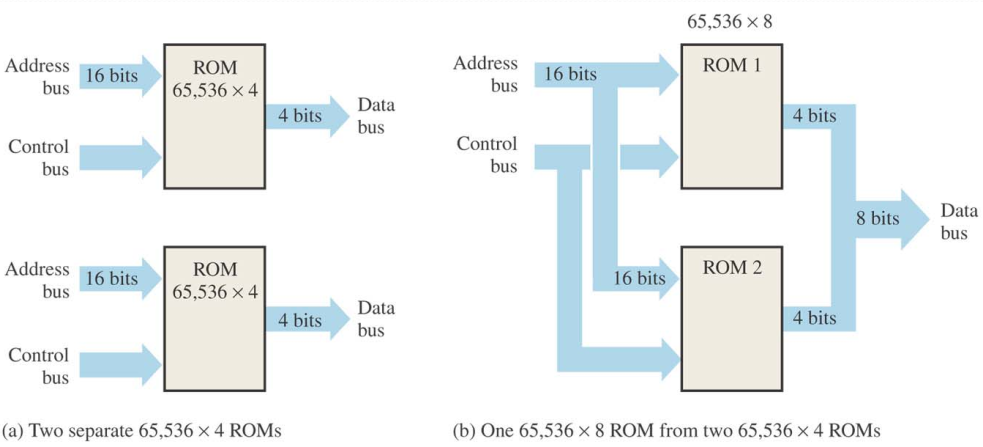
\includegraphics[width=0.6\linewidth]{fig/word-length.PNG}
	\caption{字长扩展}
\end{figure}
	\item 字容量(word-capacity)扩展
\begin{figure}[htbp]
	\centering
	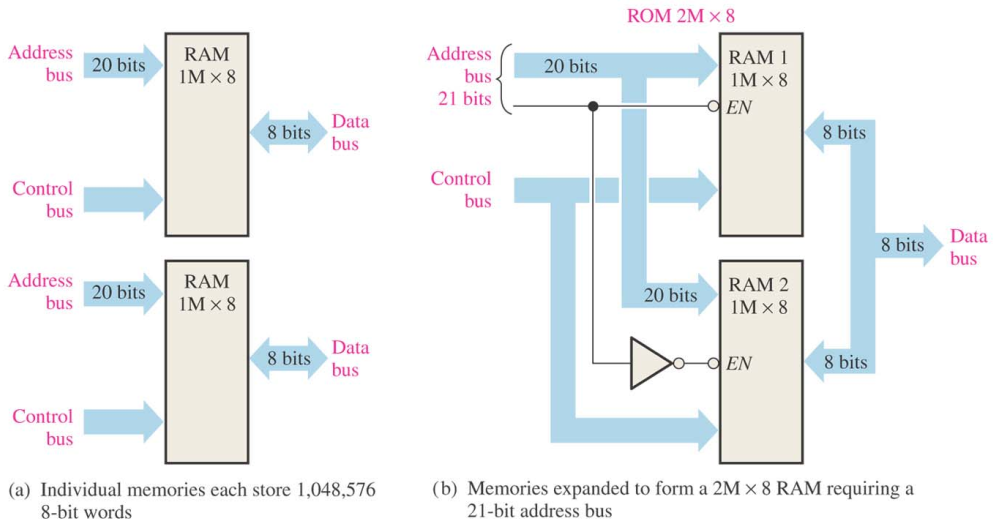
\includegraphics[width=0.6\linewidth]{fig/word-capacity.PNG}
	\caption{字容量扩展}
\end{figure}
\end{itemize}

\subsection{信号处理}
\begin{enumerate}
	\item 采样(sampling)\\
	采样频率至少是原来最高频率的两倍
	\item 滤波(filtering)\\
	奈奎斯特(Nyquist)频率等于采样频率的一半
\end{enumerate}

\subsection{其他}
\begin{figure}[htbp]
\begin{minipage}{0.5\linewidth}
	\centerline{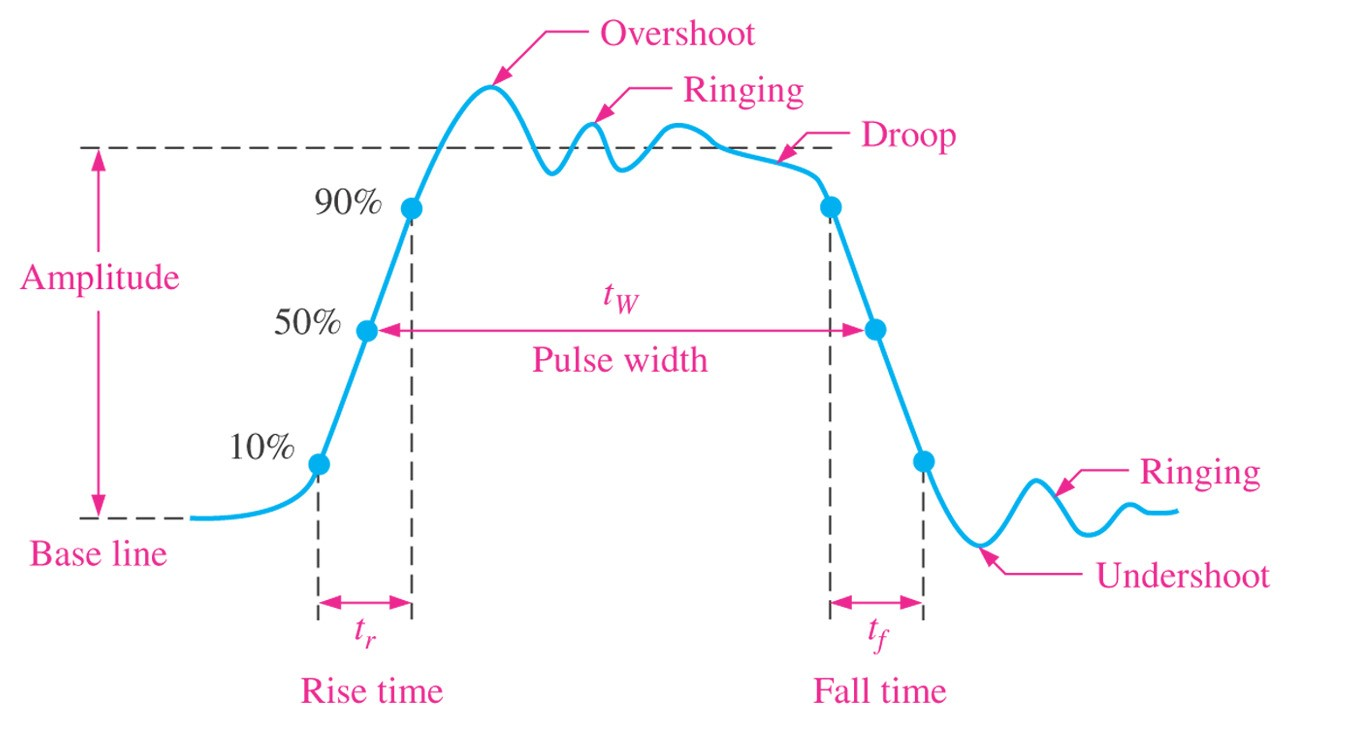
\includegraphics[width=\linewidth]{fig/nonideal_pulse_characteristics.jpg}}
	\centerline{非理想脉冲}
\end{minipage}
\begin{minipage}{0.5\linewidth}
	\centerline{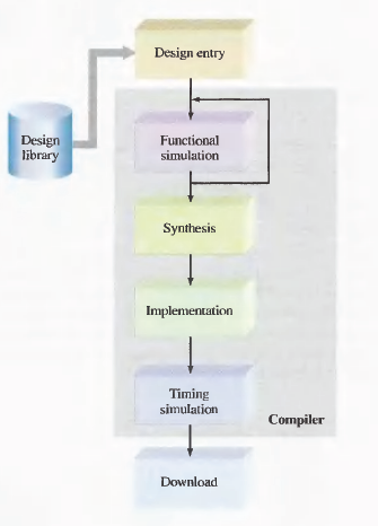
\includegraphics[width=0.6\linewidth]{fig/design_flow.png}}
	\centerline{设计流}
\end{minipage}
\end{figure}
占空比(duty cycle):$\dfrac{t_W}{T}\times 100\%$
\section{集成电路}
\begin{figure}[htbp]
	\centering
	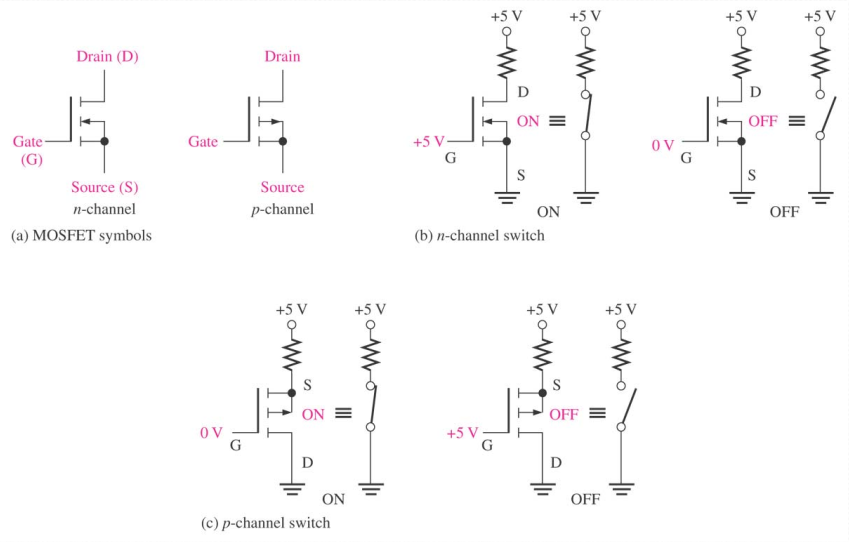
\includegraphics[width=0.8\linewidth]{fig/cmos.PNG}
	\caption{CMOS电路:\large\textbf{$n$内高,$p$外低}}
\end{figure}
\begin{figure}[htbp]
	\centering
	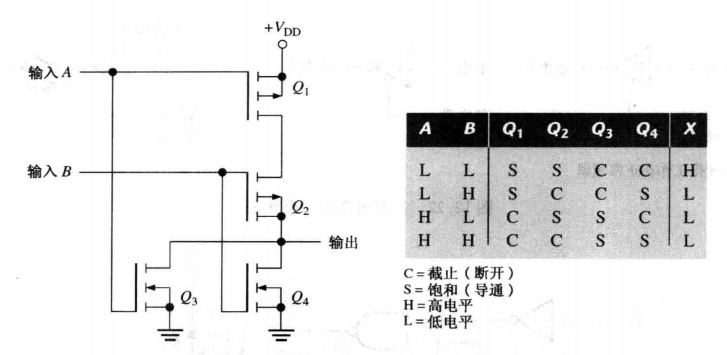
\includegraphics[width=0.6\linewidth]{fig/cmos_ex.PNG}
	\caption{CMOS或非门}
\end{figure}
\begin{figure}[htbp]
	\centering
	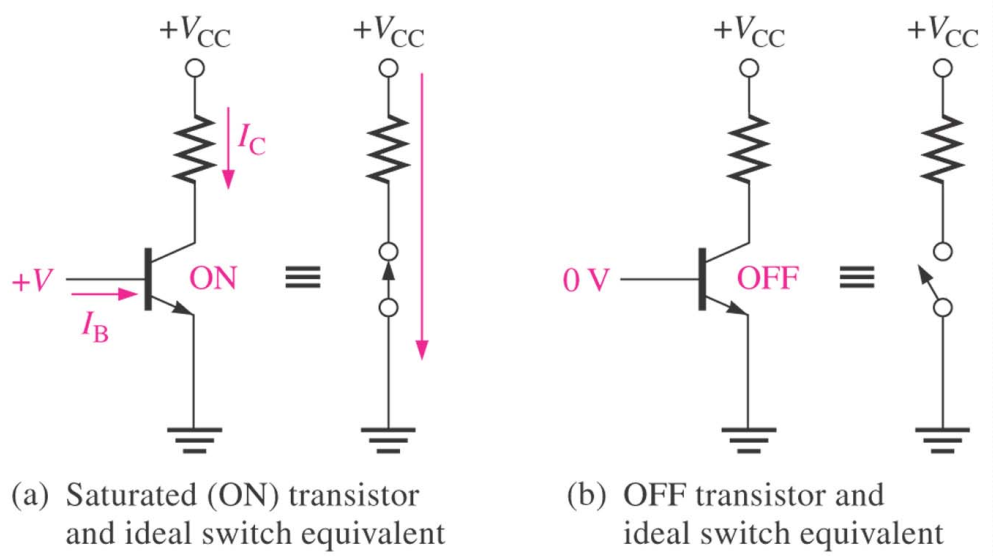
\includegraphics[width=0.6\linewidth]{fig/ttl.PNG}
	\caption{TTL电路}
\end{figure}
\begin{figure}[htbp]
\label{ttl_inverse}
	\centering
	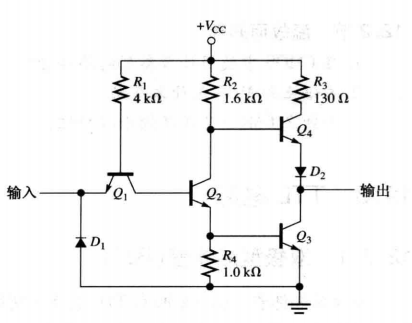
\includegraphics[width=0.6\linewidth]{fig/ttl_ex.PNG}
	\caption{TTL反相器}
\end{figure}
\par 由图\ref{ttl_inverse},$Q_1$被$V_{CC}$上拉,始终导通. 若输入为高电平,$Q_2$导通,$Q_3$导通,输出被下拉为低电平. 同时,$Q_2$在集电极处足够低的电压可以使$Q_4$截至.
\begin{figure}[htbp]
	\centering
	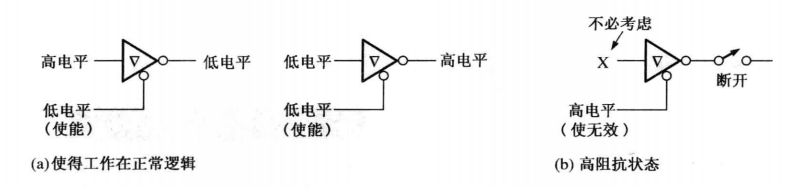
\includegraphics[width=0.6\linewidth]{fig/three_gates.PNG}
	\caption{三态门}
\end{figure}
\section{组合电路}
\subsection{基本逻辑门}
\begin{figure}[htbp]
	\centering
	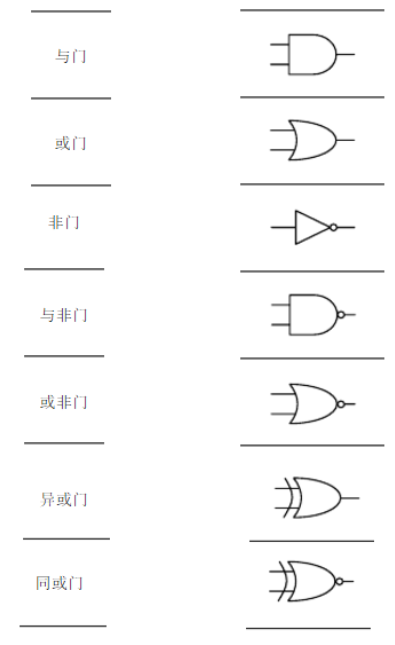
\includegraphics[width=0.6\linewidth]{fig/logic_gates.PNG}
	\caption{基本逻辑门}
\end{figure}
\subsection{布尔(Boolen)代数}
满足交换律、结合律、分配律
\[\begin{aligned}
A\ol{A}&=0 \qquad &A+\ol{A}&=1\\
A\ol{B}+\ol{A}B&=A\oplus B \qquad &AB+\ol{A}\ol{B}&=A\odot B
\end{aligned}\]
\[\begin{aligned}
A+BC&=A(1+B+C)+BC \qquad &A+\ol{A}B&=A(1+B)+\ol{A}B\\
&=(A+B)(A+C)\qquad & &=A+B
\end{aligned}\]

\subsection{卡诺(Karnaugh)图}
\begin{figure}[htbp]
	\centering
	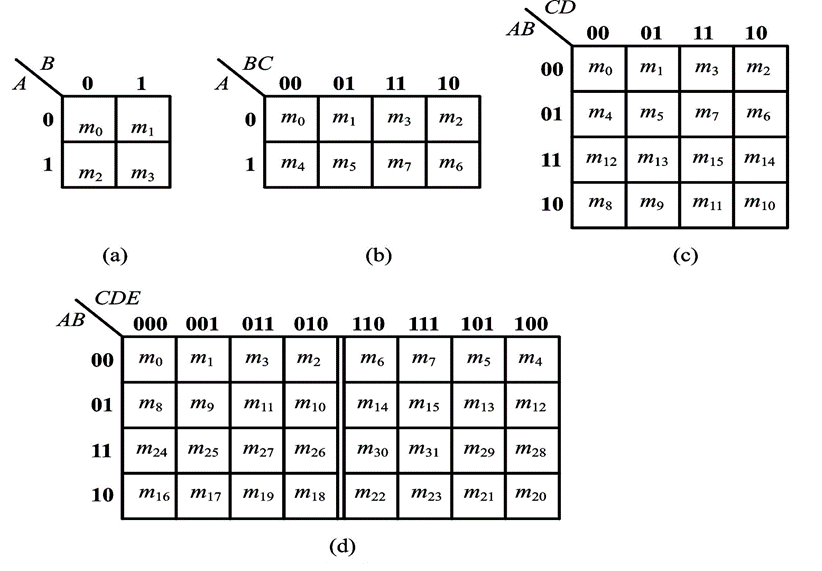
\includegraphics[width=0.8\linewidth]{fig/Karnaugh_graph.png}
	\caption{不同阶卡诺图}
\end{figure}
\begin{figure}[htbp]
	\centering
	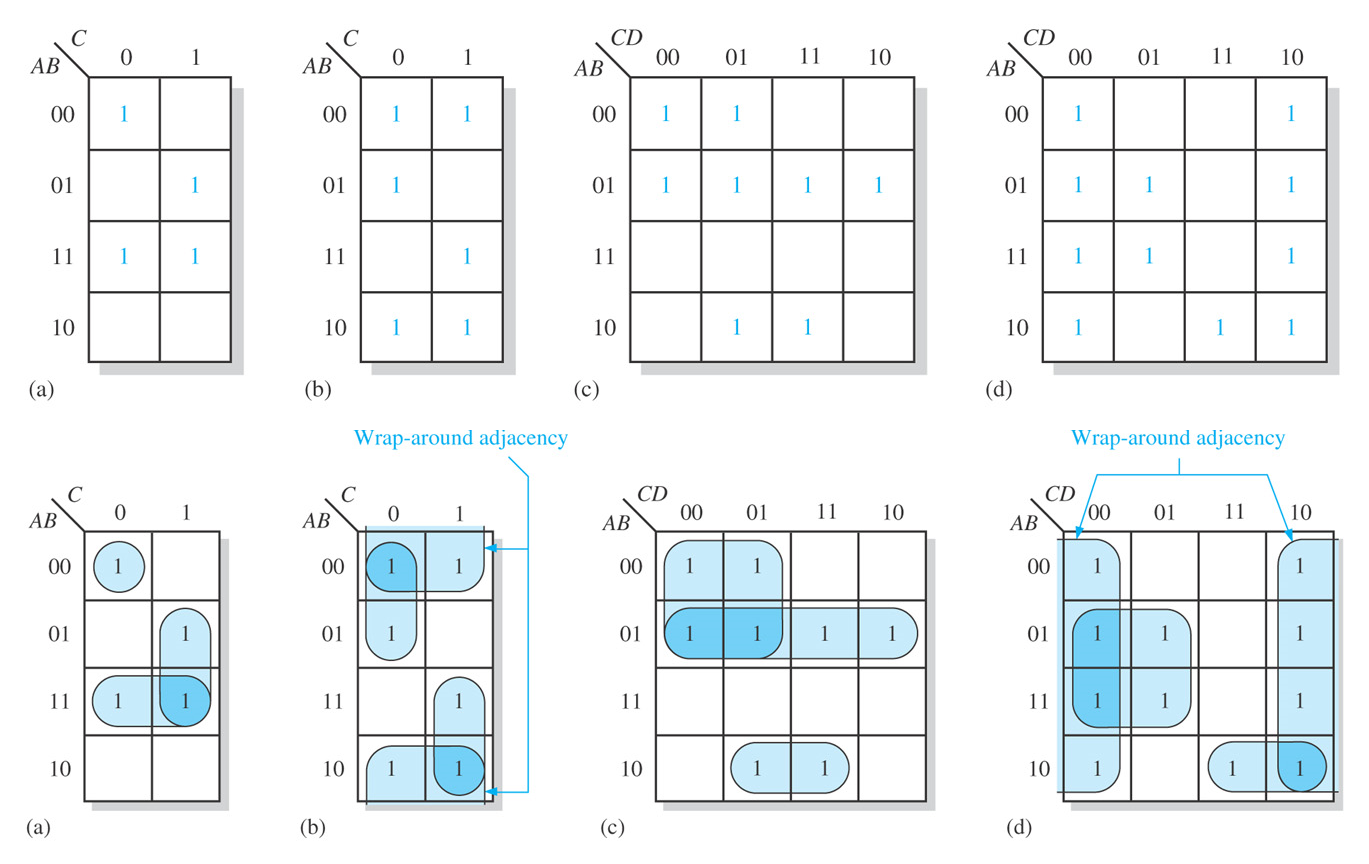
\includegraphics[width=0.8\linewidth]{fig/Karnaugh_example.png}
	\caption{Sum of Product(SOP)化简}
\end{figure}

\subsection{功能器件}
\subsubsection{加法器}
\begin{figure}[htbp]
	\centering
	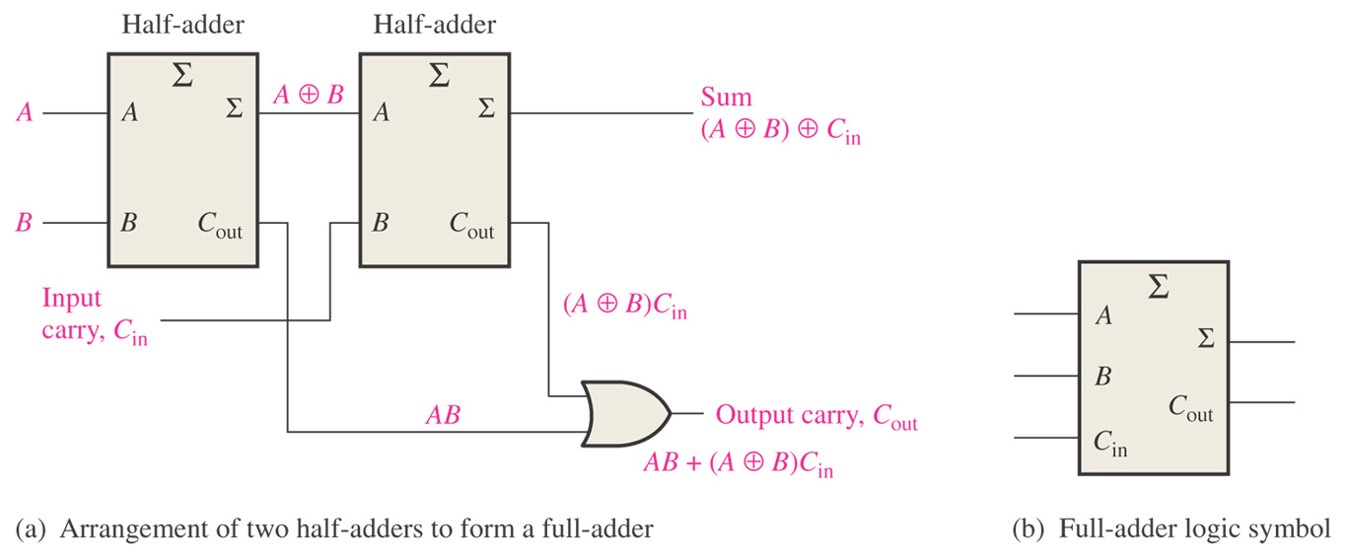
\includegraphics[width=0.8\linewidth]{fig/adder.jpg}
	\caption{半加法器与全加法器}
\end{figure}
\begin{figure}[htbp]
	\centering
	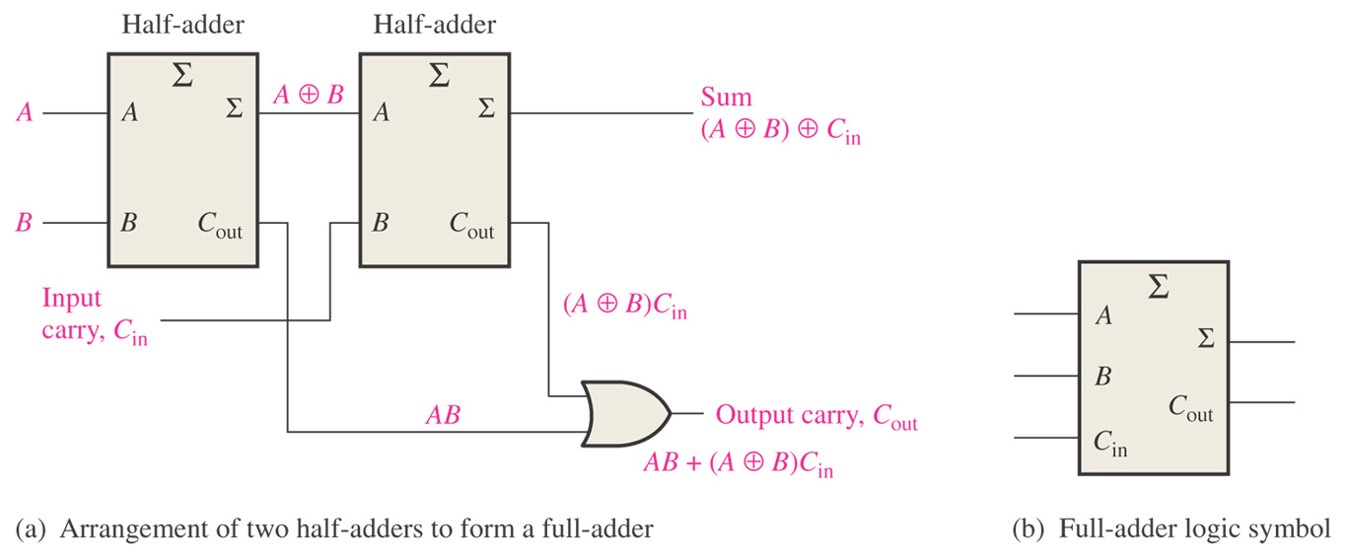
\includegraphics[width=0.8\linewidth]{fig/adder.jpg}
	\caption{异步加法器改造为同步加法器}
\end{figure}
\[\begin{aligned}
&\text{Carry generation: }&C_g&=AB\\
&\text{Carry propagation: }&C_g&=AB\\
&\text{Output carry: }&C_g&=AB\\
& &C_{in2}&=C_{out1}=C_{g1}+C_{p1}C_{in1}\\
& &C_{in3}&=C_{out2}=C_{g2}+C_{p2}C_{in2}=C_{g2}+C_{p2}(C_{g1}+C_{p1}C_{in1})
\end{aligned}\]
\subsubsection{比较器(Comparator)}
\begin{figure}[htbp]
	\centering
	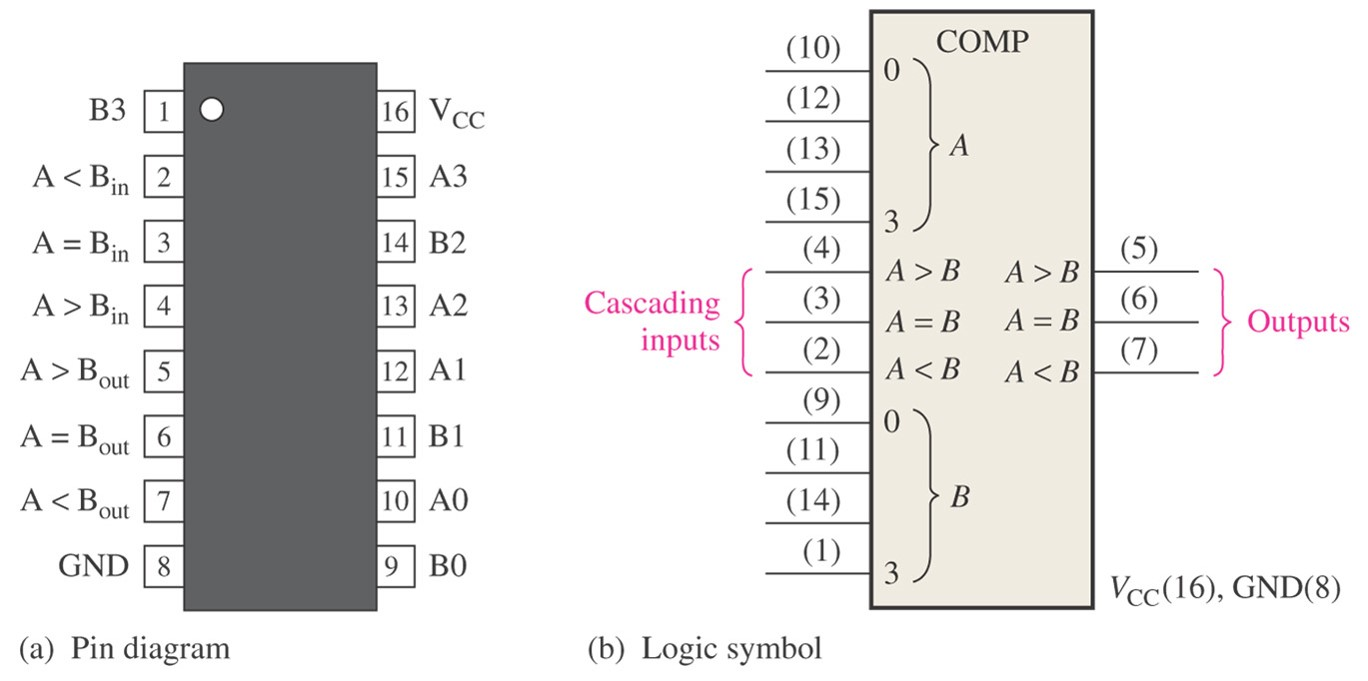
\includegraphics[width=0.8\linewidth]{fig/comparator.jpg}
	\caption{比较器}
\end{figure}
\subsubsection{译码器(Decoder)}
BCD码转对应端口输出,注意输出是反的
\begin{figure}[htbp]
	\centering
	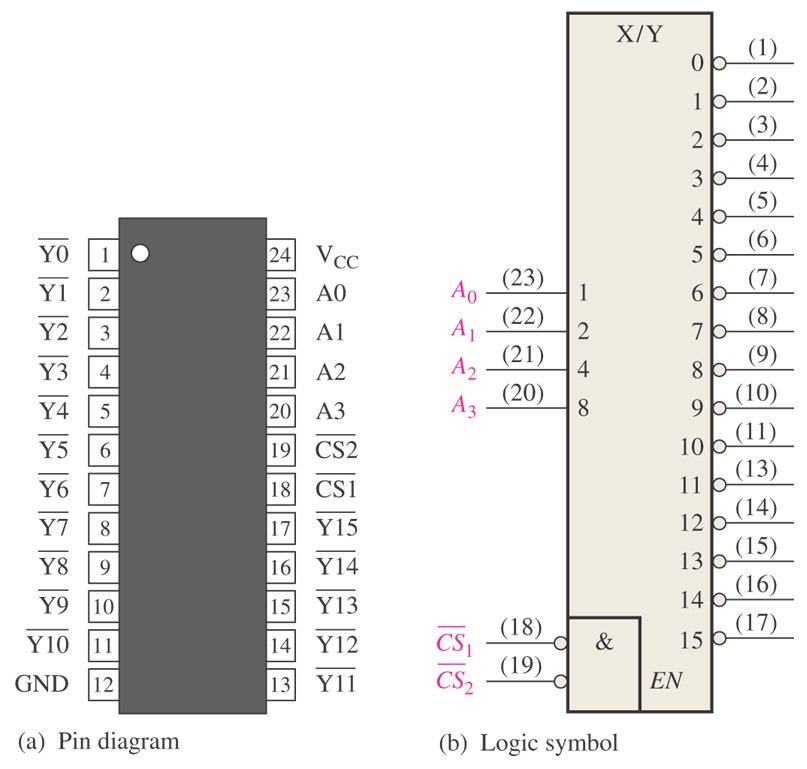
\includegraphics[width=0.5\linewidth]{fig/decoder.jpg}
	\caption{译码器}
\end{figure}
\par BCD转7段数码管
\begin{enumerate}
	\item 共阴(cathode):高电平亮
	\item 共阳(anode):低电平亮
\end{enumerate}
\subsubsection{编码器(Encoder)}
输入转BCD码
\begin{figure}[htbp]
	\centering
	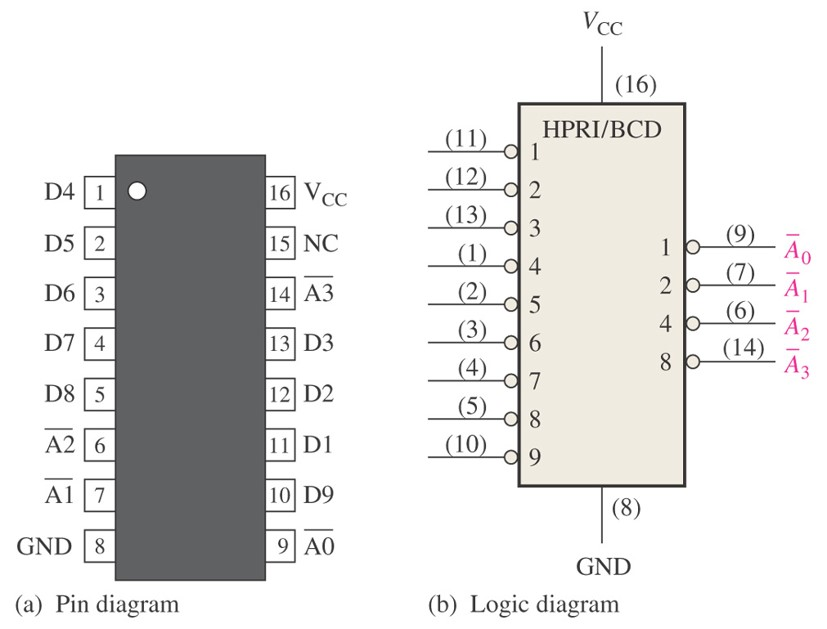
\includegraphics[width=0.6\linewidth]{fig/encoder.jpg}
	\caption{编码器}
\end{figure}
\subsubsection{选择器(Multiplexer)}
通过BCD码选择对应路输出
\begin{figure}[htbp]
	\centering
	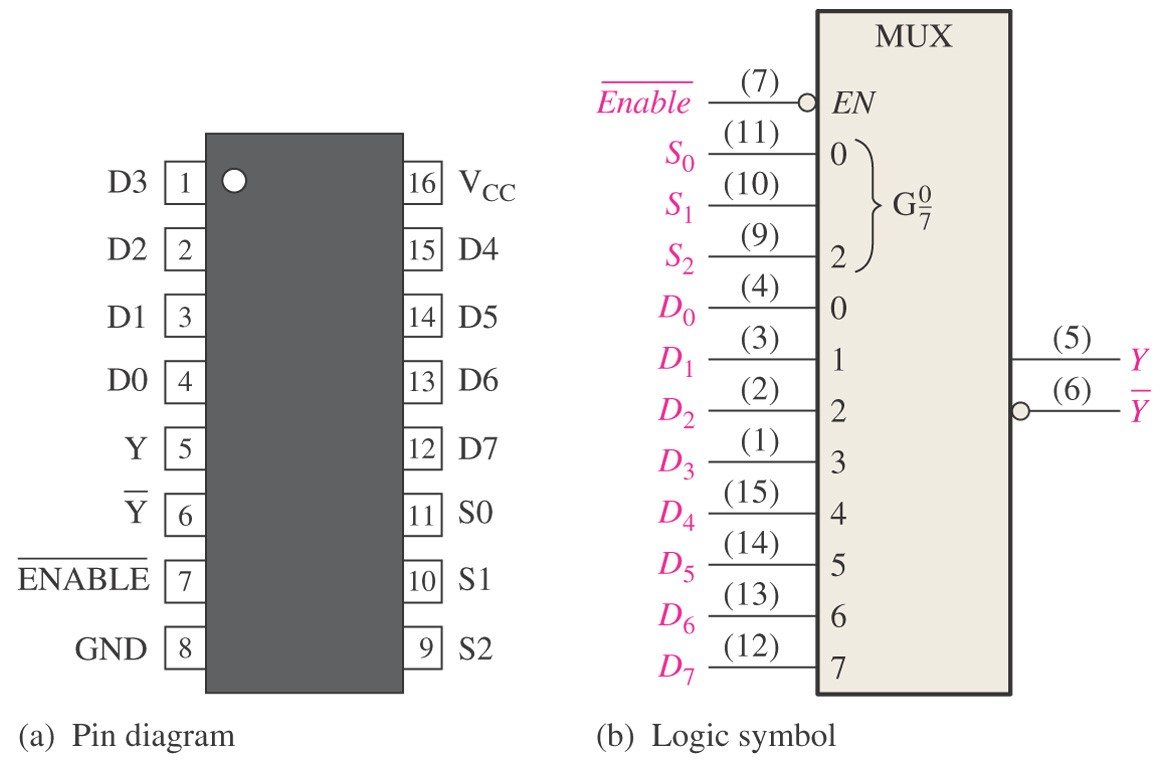
\includegraphics[width=0.6\linewidth]{fig/multiplexer.jpg}
	\caption{选择器}
\end{figure}
\subsubsection{多路分配器(Demultiplexer)}
将对应输入分配到对应输出路

\subsection{竞争与冒险}
\begin{enumerate}
	\item 竞争(race):输入到输出途径不同,延时时间不同,到达输出的时间不同
	\item 冒险(hazard):竞争结果导致逻辑电路产生错误输出
\end{enumerate}
\par 如$F=AB+\ol{A}C$,因为取非,导致两条道路时间不同,使得输出出现毛刺现象
\par 可加入冗余项以避免冒险,如改成$F=AB+\ol{A}C+BC$
\section{时序电路}
\subsection{锁存器}
\par 用于存储数据
\begin{figure}[htbp]
	\centering
	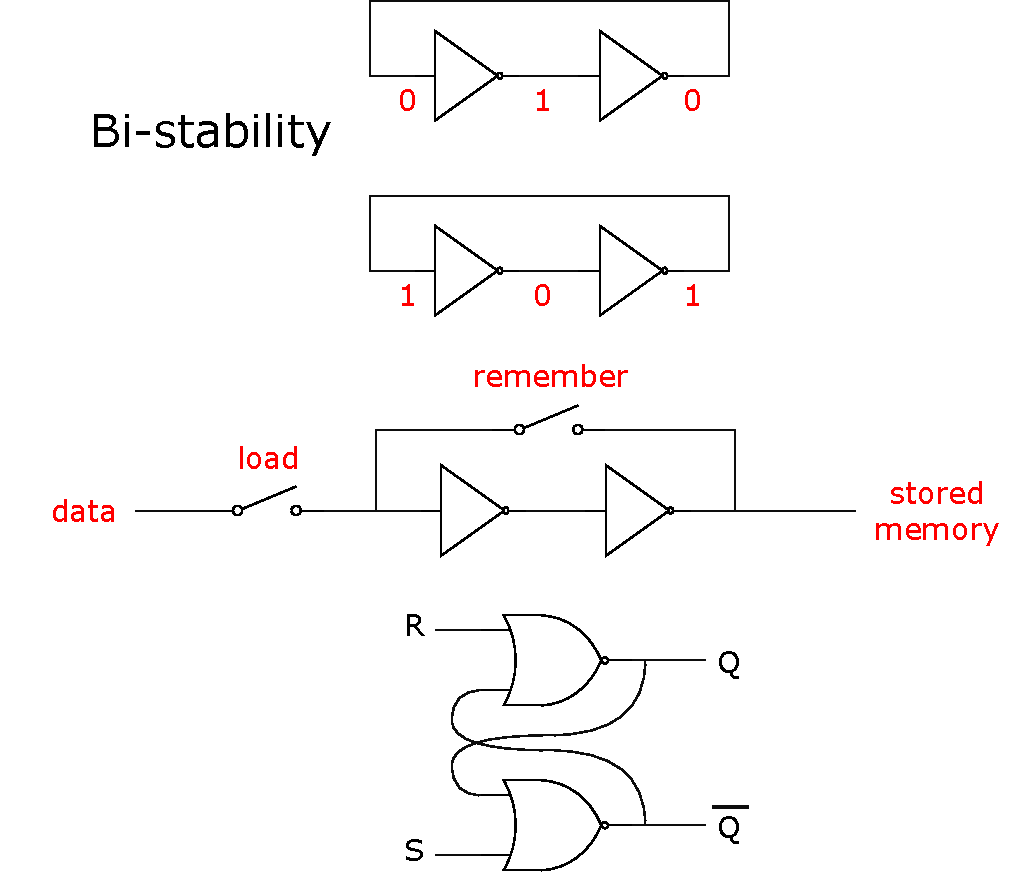
\includegraphics[width=0.6\linewidth]{fig/latches.pdf}
	\caption{SR锁存器(latch)}
\end{figure}
\par SR锁存器状态表
\begin{center}
\begin{tabular}{|c|c|c|c|}
\hline
S & R & 状态\\\hline
0 & 0 & 不变\\\hline
0 & 1 & 复位\\\hline
1 & 0 & 置位\\\hline
1 & 1 & N/A\\\hline
\end{tabular}
\end{center}
\par D锁存器状态:0复位,1置位
\par 门(选通端):决定是否运作

\subsection{触发器}
\subsubsection{SR/D触发器}
\par 触发器状态变化与锁存器相同
\begin{figure}[htbp]
	\centering
	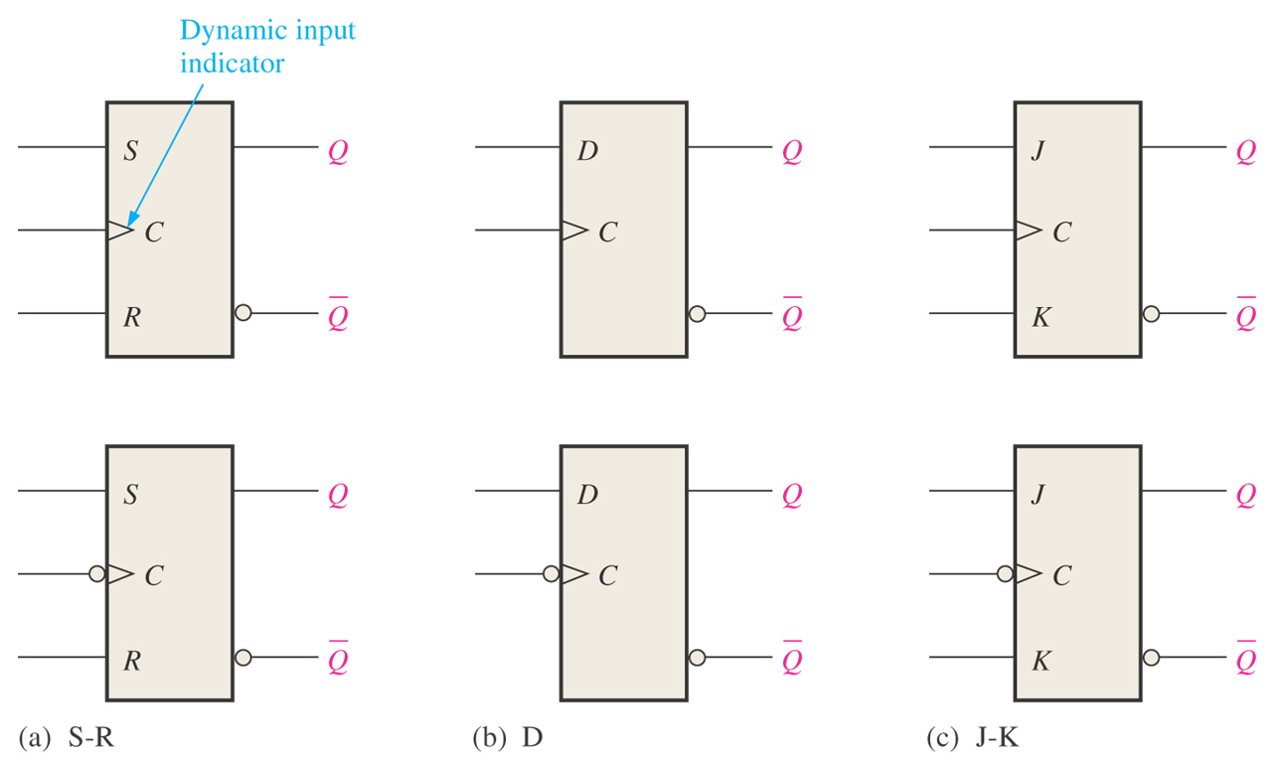
\includegraphics[width=0.6\linewidth]{fig/flip-flops.png}
	\caption{触发器}
\end{figure}
边缘触发其实通过竞争实现(如输入加一个与门后与非$\ol{A\ol{A}}$)
\subsubsection{JK触发器}
\begin{figure}[htbp]
	\centering
	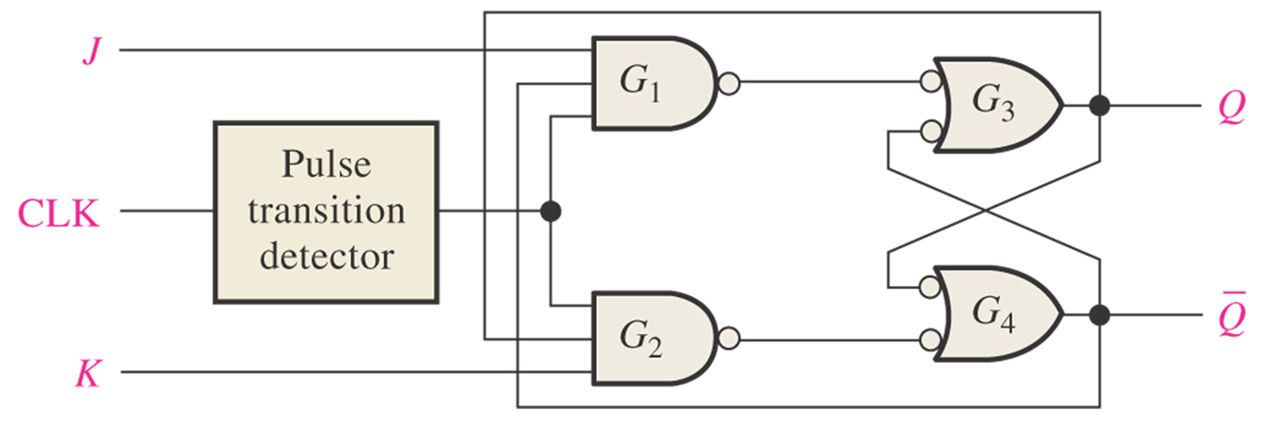
\includegraphics[width=0.6\linewidth]{fig/JK_flip-flop.png}
	\caption{JK触发器}
\end{figure}
\par JK触发器状态表
\begin{center}
\begin{tabular}{|c|c|c|c|}
\hline
J & K & 状态\\\hline
0 & 0 & 不变\\\hline
0 & 1 & 复位\\\hline
1 & 0 & 置位\\\hline
1 & 1 & 转换\\\hline
\end{tabular}
\end{center}
\par 注意看有无\textcolor{red}{bubble},看是上升沿还是下降沿
\subsubsection{应用}
\begin{enumerate}
	\item 并行数据传输:接同一时钟
	\item 分频:JK均接高,遇上升沿才触发,故可实现
\begin{figure}[htbp]
	\centering
	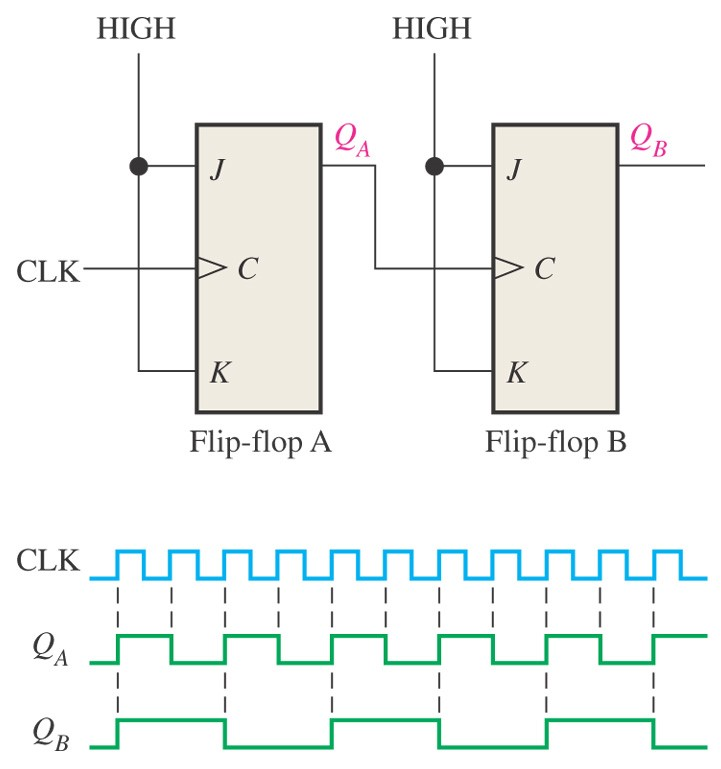
\includegraphics[width=0.4\linewidth]{fig/frequency_divisor.jpg}
	\caption{分频器}
\end{figure}
	\item 计数器:也相当于分频
\begin{figure}[htbp]
	\centering
	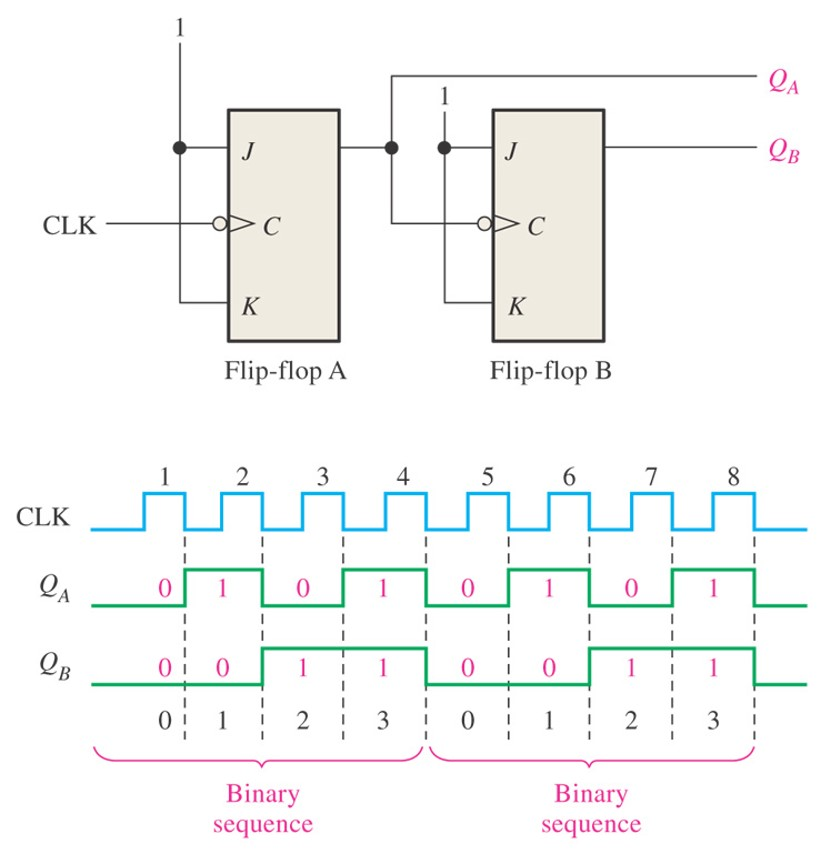
\includegraphics[width=0.4\linewidth]{fig/counter.jpg}
	\caption{计数器}
\end{figure}
\end{enumerate}

\subsection{单稳态触发器}
\begin{figure}[htbp]
	\centering
	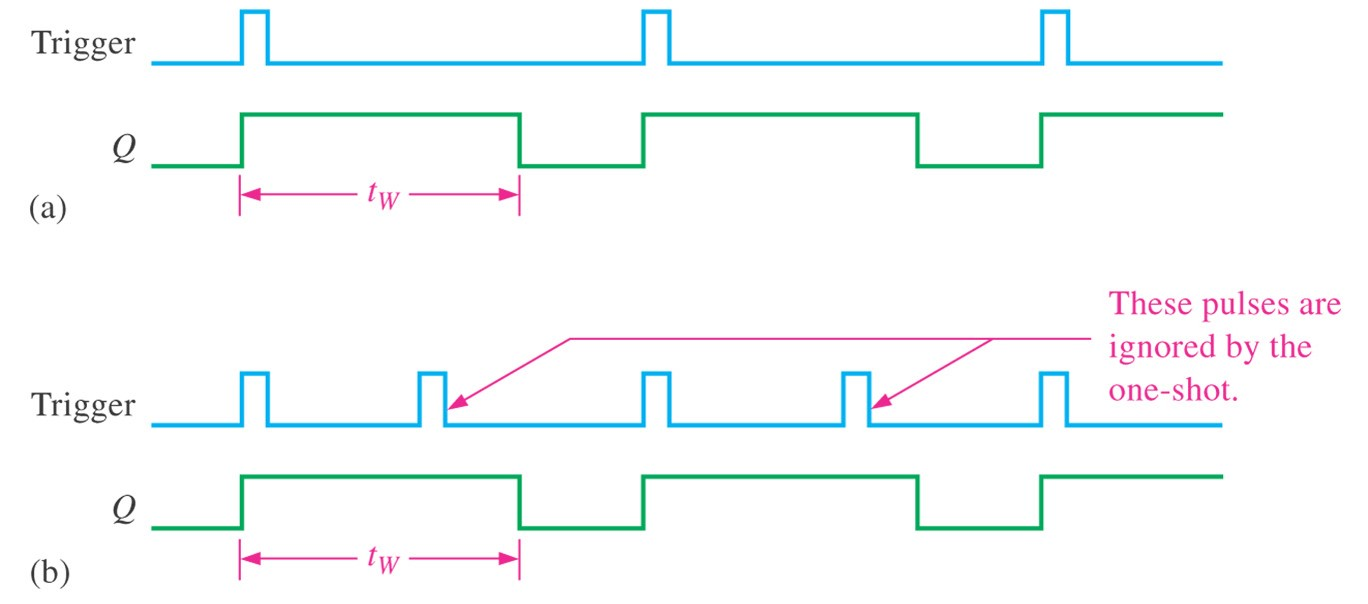
\includegraphics[width=0.6\linewidth]{fig/one-shot.jpg}
	\caption{单稳态触发器(不可重复触发)}
\end{figure}

\subsection{555计时器}
\begin{itemize}
	\item 单稳态触发器(mono-stable one-shot)
	\item 非稳态多谐振荡器(astable multi-vibration oscillator)
\end{itemize}
\begin{figure}[htbp]
	\centering
	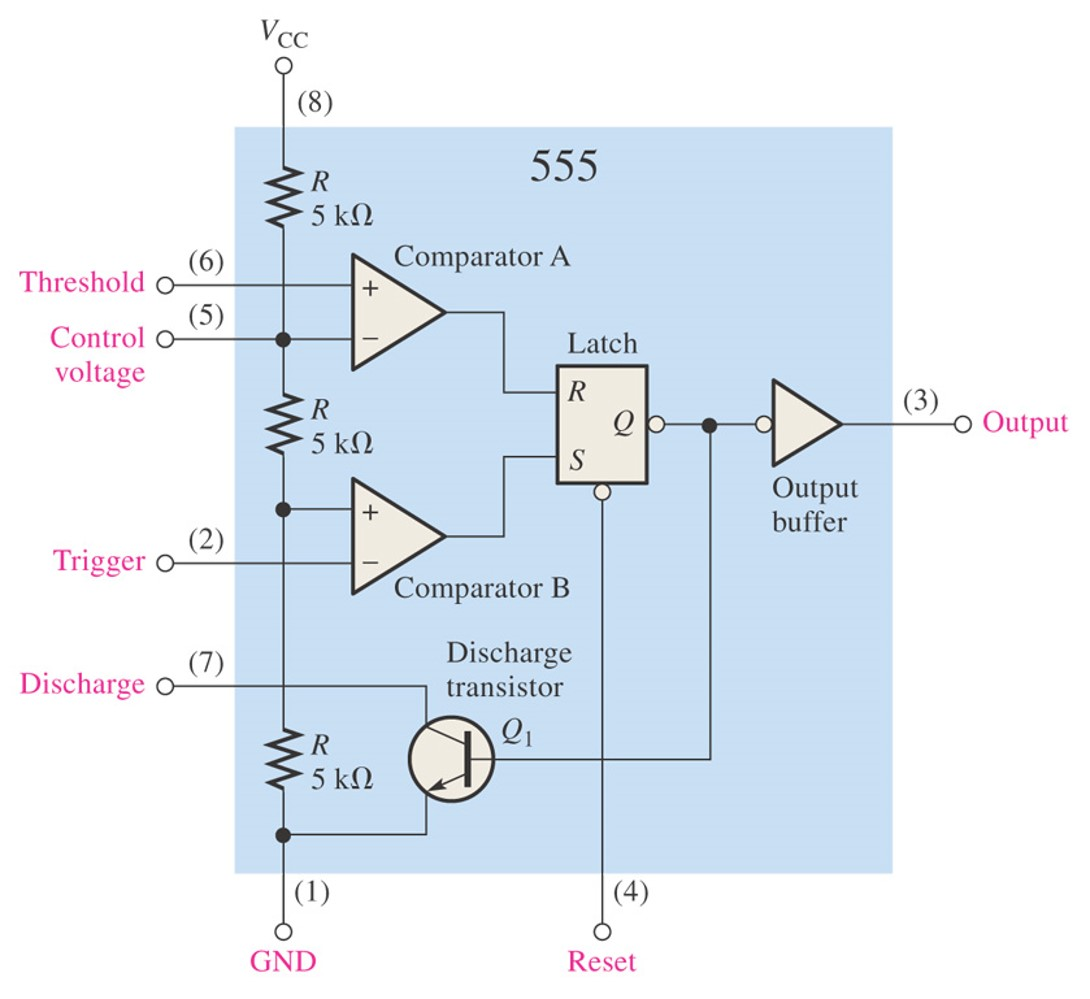
\includegraphics[width=0.6\linewidth]{fig/555timer.jpg}
	\caption{555计时器}
\end{figure}
\[f=\dfrac{1.44}{(R_1+2R_2)C_1}\]
\[DC=\dfrac{R_1+R_2}{R_1+2R_2}\times 100\%\]

\subsection{移位寄存器}
\subsubsection{约翰逊计数器}
\begin{figure}[htbp]
	\centering
	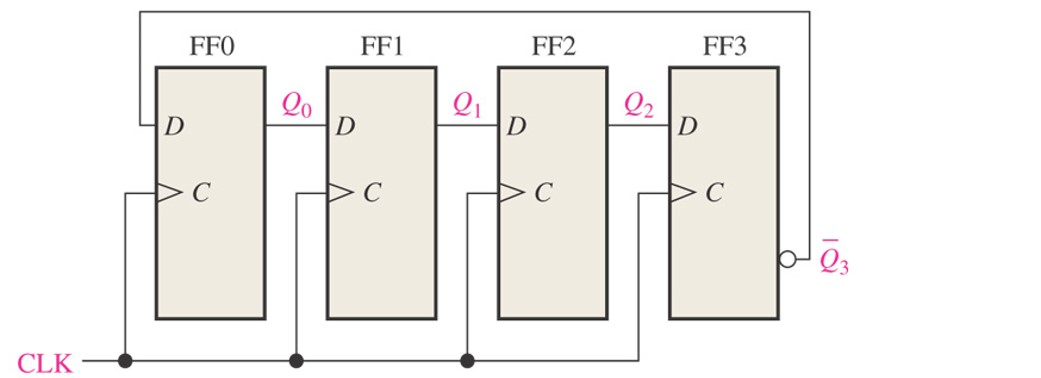
\includegraphics[width=0.6\linewidth]{fig/johnson.jpg}
	\caption{约翰逊(Johnson)计数器}
\end{figure}
\par 计数范围$M=2N$
\begin{center}
\begin{tabular}{|c|c|c|c|c|}
\hline
计数 & $Q_0$ & $Q_1$ & $Q_2$ & $Q_3$\\\hline
0 & 0 & 0 & 0 & 0\\\hline
1 & 1 & 0 & 0 & 0\\\hline
2 & 1 & 1 & 0 & 0\\\hline
3 & 1 & 1 & 1 & 0\\\hline
4 & 1 & 1 & 1 & 1\\\hline
5 & 0 & 1 & 1 & 1\\\hline
6 & 0 & 0 & 1 & 1\\\hline
7 & 0 & 0 & 0 & 1\\\hline
\end{tabular}
\end{center}
\subsubsection{环计数器}
\par 计数范围$M=N$
\begin{figure}[htbp]
	\centering
	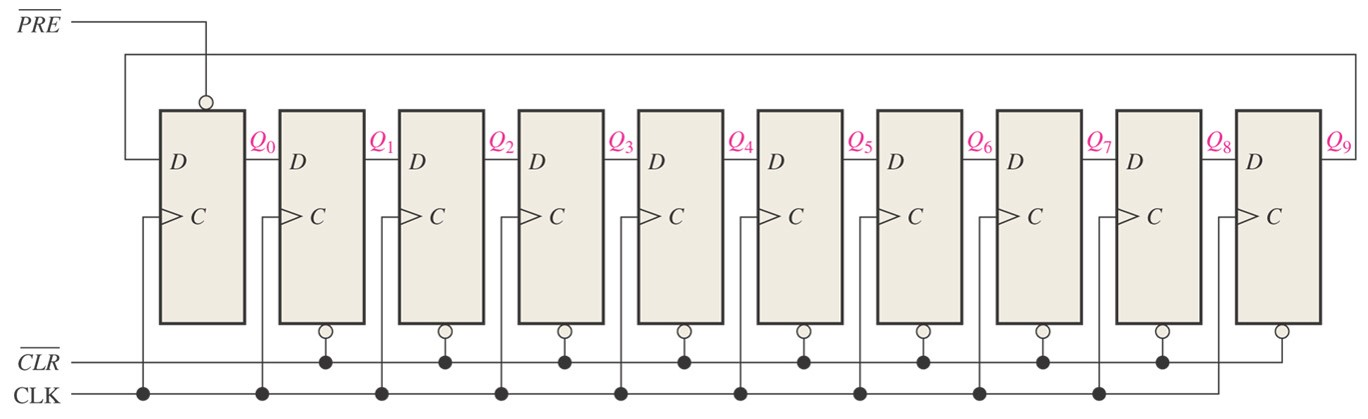
\includegraphics[width=0.6\linewidth]{fig/ring_counter.jpg}
	\caption{环计数器}
\end{figure}
\par 初始置为$1000000000$

\subsection{计数器}
\subsubsection{同步异步计数器}
\begin{figure}[htbp]
	\centering
	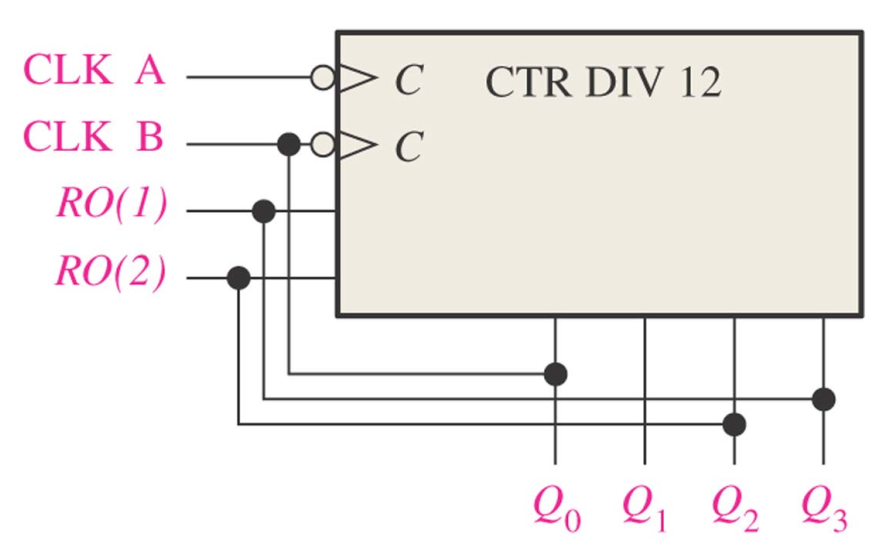
\includegraphics[width=0.3\linewidth]{fig/74ls93.PNG}
	\caption{16进制计数器}
\end{figure}
\par RO(1)与RO(2)同时为高时清零,CLK A控制二进制计数器($Q_0$),CLK B控制八进制计数器($Q_1\thicksim Q_3$),故将$Q_0$输出与八进制计数器相连可得十六进制计数器
\begin{figure}[htbp]
	\centering
	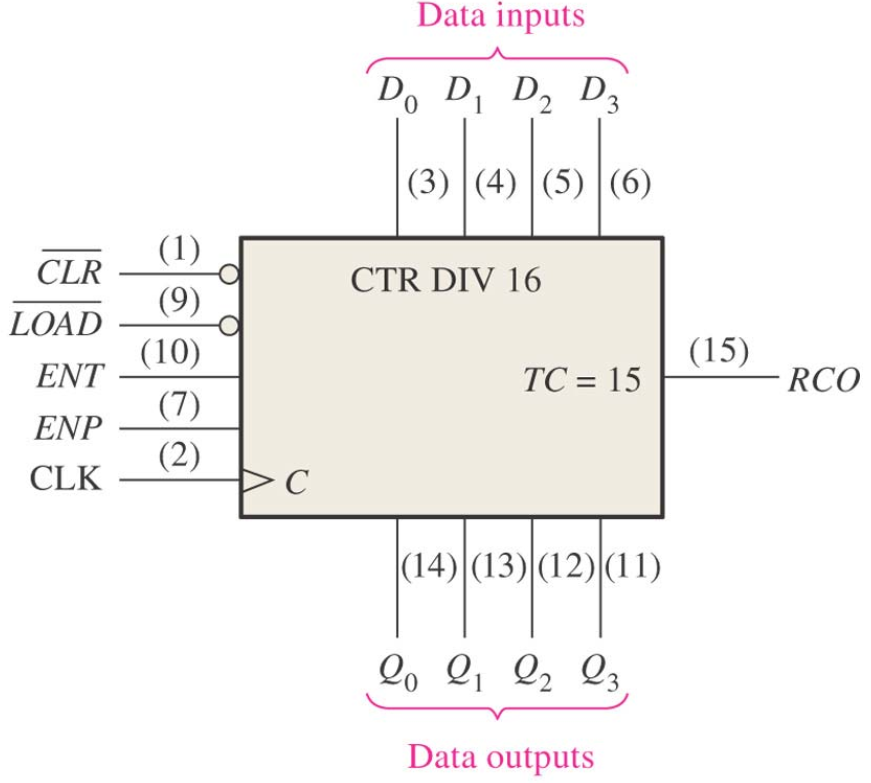
\includegraphics[width=0.3\linewidth]{fig/74hc163.PNG}
	\caption{4位同步二进制计数器}
\end{figure}
\par $\ol{LOAD}$为低时读取数据,ENT、ENP为使能端,同时高电平有效,RCO为进位端
\subsubsection{应用}
\begin{figure}[htbp]
	\centering
	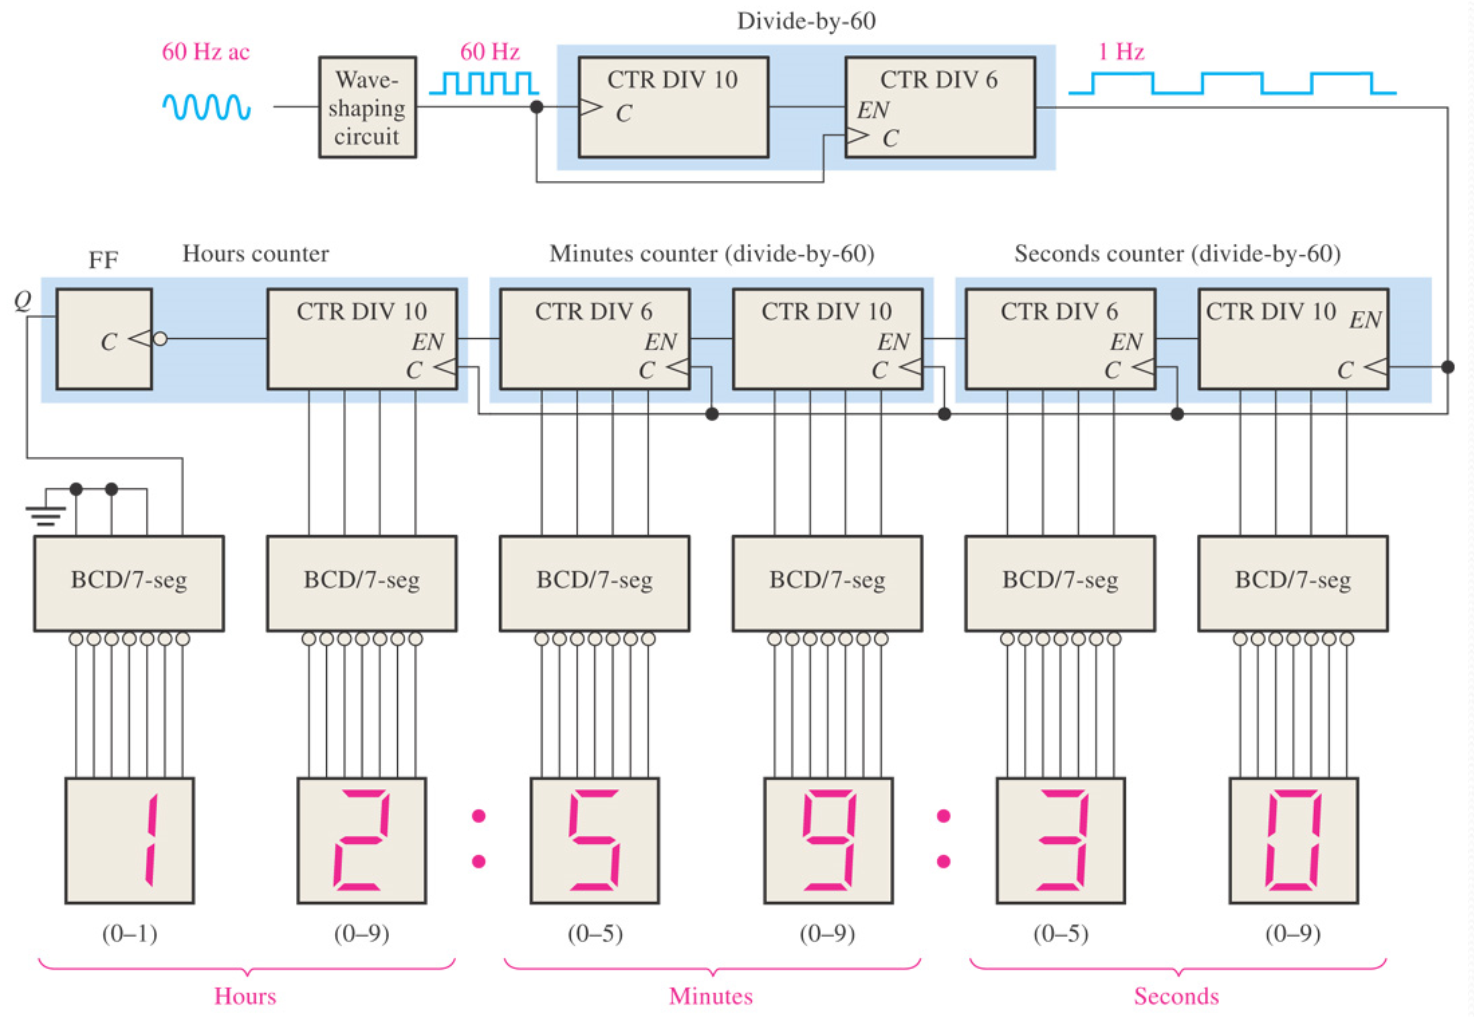
\includegraphics[width=0.6\linewidth]{fig/timer.PNG}
	\caption{时钟}
\end{figure}
\section{电路设计}
\subsection{电路分类}
\begin{enumerate}
\item 摩尔(Moore)电路
\begin{figure}[htbp]
	\centering
	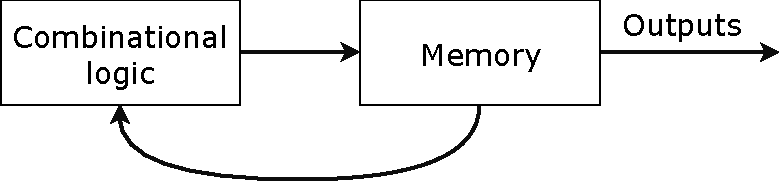
\includegraphics[width=0.4\linewidth]{fig/moore_machine.pdf}
	\caption{触发器}
\end{figure}
\item 米勒(Mealy)电路
\begin{figure}[htbp]
	\centering
	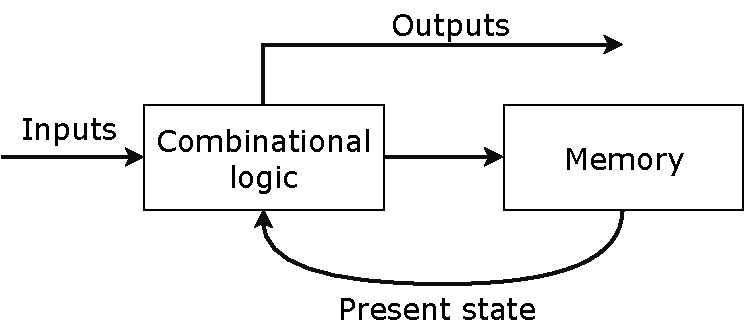
\includegraphics[width=0.4\linewidth]{fig/mealy_machine.pdf}
	\caption{触发器}
\end{figure}
\end{enumerate}
\subsection{设计步骤}
\par 基于状态转移表格的方法
\begin{enumerate}
    \item 状态图
    \item 次态表
    \item 触发器转移表
\begin{center}
\begin{tabular}{|c|c|c|c|}
\hline
$Q^n$ & $Q^{n+1}$ & J & K\\\hline
0 & 0 & 0 & X\\\hline
0 & 1 & 1 & X\\\hline
1 & 0 & X & 1\\\hline
1 & 1 & X & 0\\\hline
\end{tabular}
\end{center}
    \item 触发器JK卡诺图
    \item JK驱动方程
    \item 时序电路
\end{enumerate}
\par 基于状态方程的方法
\begin{enumerate}
	\item 状态表
	\item 次态卡诺图
	\item 状态方程 $Q^{n+1}=J\ol{Q^n}+\ol{K}Q^n$
	\item 驱动方程
	\item 时序电路
\end{enumerate}
\subsection{实例操作}
\par 目的:用JK触发器实现一个12进制同步计数器
\begin{enumerate}
    \item 状态转换图
    \begin{figure}[H]
        \centering
        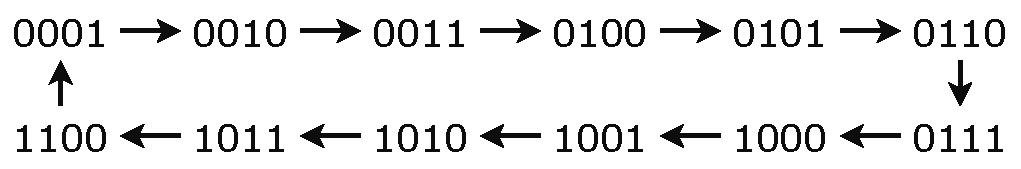
\includegraphics[width=0.7\linewidth]{fig/12system_state.pdf}
    \end{figure}
    \item 确定电路所需触发器数目\\
    由于$2^4=16>12$,故需要$4$个JK触发器
    \item 次态卡诺图
    \begin{figure}[H]
        \centering
        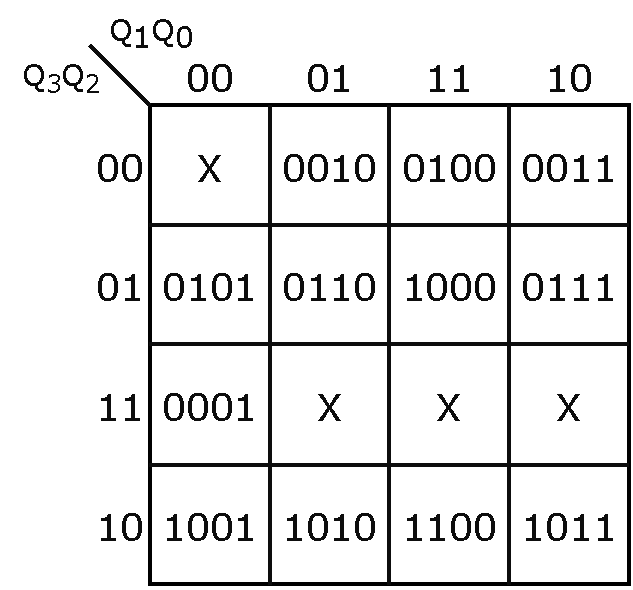
\includegraphics[width=0.4\linewidth]{fig/Karnaugh_12system.pdf}
    \end{figure}
    \item 触发器状态方程,由卡诺图可得
    \[\begin{aligned}
    Q_0^{n+1}&=\overline{Q_0}\\
    Q_1^{n+1}&=Q_0\overline{Q_1}+\overline{Q_0}Q_1\\
    Q_2^{n+1}&=Q_0Q_1\ol{Q_2}+\ol{Q_1}Q_2\ol{Q_3}+\ol{Q_0}Q_2\ol{Q_3}\\
    Q_3^{n+1}&=\ol{Q_2}Q_3+Q_0Q_1Q_2\ol{Q_3}
    \end{aligned}\]
    \item 触发器驱动方程,由
    \[Q^{n+1}=J\ol{Q^n}+\ol{K}Q^n\]
    将状态方程整理为上式形式,可得
    \[\begin{aligned}
    J_0&=1 \qquad &K_0&=1\\
    J_1&=Q_0 \qquad &K_0&=Q_0\\
    J_2&=Q_1Q_0 \qquad &K_2&=\ol{\ol{Q_3}\ol{Q_1}+\ol{Q_3}\ol{Q_0}}=\ol{Q_3}+Q_1Q_0\\
    J_3&=Q_2Q_1Q_0 \qquad &K_3&=Q_2
    \end{aligned}\]
    \item 检查自启动\\
    当输入为1111和0000时,可自动跳转至0001;输入为1101时,跳转至0010;输入为1110时,跳转至0011
\end{enumerate}
\par Proteus电路图连接如下
\begin{figure}[H]
    \centering
    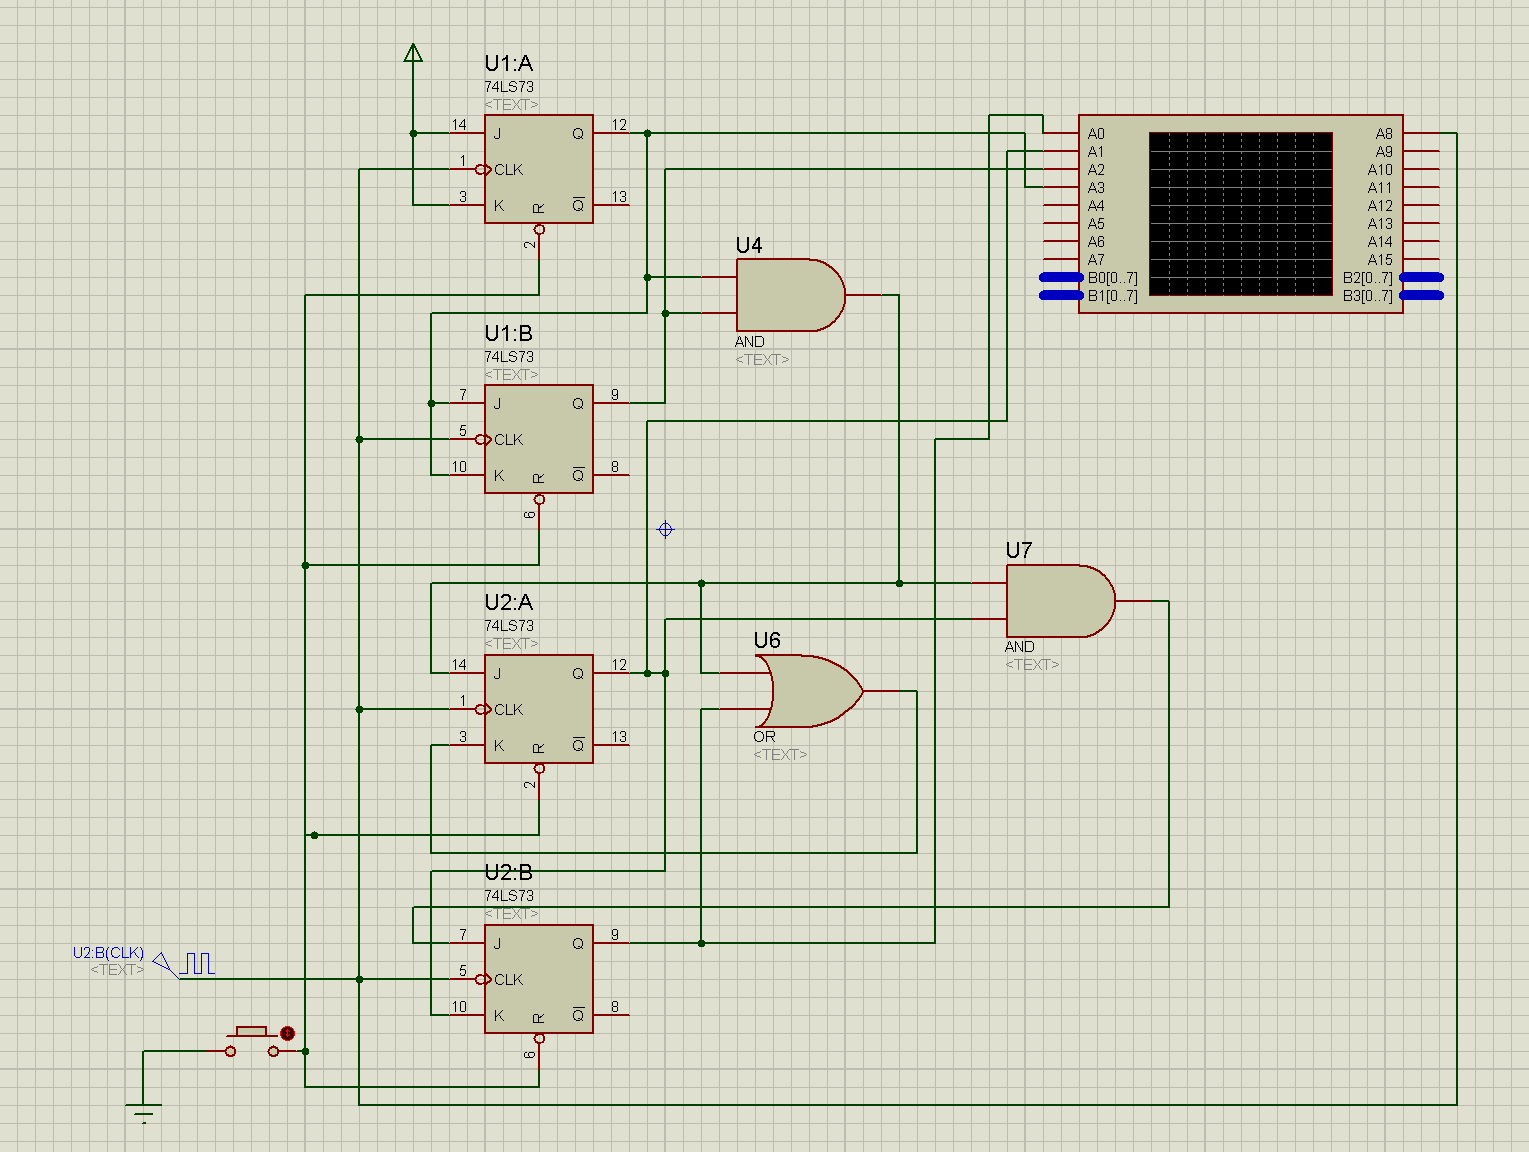
\includegraphics[width=0.9\linewidth]{fig/12system_protues.PNG}
\end{figure}
\par 仿真结果如下
\begin{figure}[H]
    \centering
    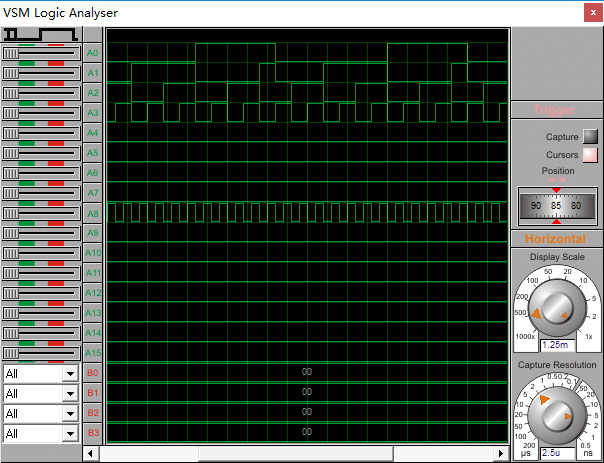
\includegraphics[width=0.6\linewidth]{fig/12system_wave.PNG}
\end{figure}

\end{document}